\documentclass[
  bibliography=totoc,     % Literatur im Inhaltsverzeichnis
  captions=tableheading,  % Tabellenüberschriften
  titlepage=firstiscover, % Titelseite ist Deckblatt
]{scrartcl}

% Paket float verbessern
\usepackage{scrhack}

% Warnung, falls nochmal kompiliert werden muss
\usepackage[aux]{rerunfilecheck}

% unverzichtbare Mathe-Befehle
\usepackage{amsmath}
% viele Mathe-Symbole
\usepackage{amssymb}
% Erweiterungen für amsmath
\usepackage{mathtools}

% Fonteinstellungen
\usepackage{fontspec}
% Latin Modern Fonts werden automatisch geladen
% Alternativ zum Beispiel:
%\setromanfont{Libertinus Serif}
%\setsansfont{Libertinus Sans}
%\setmonofont{Libertinus Mono}

% Wenn man andere Schriftarten gesetzt hat,
% sollte man das Seiten-Layout neu berechnen lassen
\recalctypearea{}

% deutsche Spracheinstellungen
\usepackage[ngerman]{babel}


\usepackage[
  math-style=ISO,    % ┐
  bold-style=ISO,    % │
  sans-style=italic, % │ ISO-Standard folgen
  nabla=upright,     % │
  partial=upright,   % │
  mathrm=sym,        % ┘
  warnings-off={           % ┐
    mathtools-colon,       % │ unnötige Warnungen ausschalten
    mathtools-overbracket, % │
  },                       % ┘
]{unicode-math}

% traditionelle Fonts für Mathematik
\setmathfont{Latin Modern Math}
% Alternativ zum Beispiel:
%\setmathfont{Libertinus Math}

\setmathfont{XITS Math}[range={scr, bfscr}]
\setmathfont{XITS Math}[range={cal, bfcal}, StylisticSet=1]

% Zahlen und Einheiten
\usepackage[
  locale=DE,                   % deutsche Einstellungen
  separate-uncertainty=true,   % immer Unsicherheit mit \pm
  per-mode=symbol-or-fraction, % / in inline math, fraction in display math
]{siunitx}

% chemische Formeln
\usepackage[
  version=4,
  math-greek=default, % ┐ mit unicode-math zusammenarbeiten
  text-greek=default, % ┘
]{mhchem}

% richtige Anführungszeichen
\usepackage[autostyle]{csquotes}

% schöne Brüche im Text
\usepackage{xfrac}

% Standardplatzierung für Floats einstellen
\usepackage{float}
\floatplacement{figure}{htbp}
\floatplacement{table}{htbp}

% Floats innerhalb einer Section halten
\usepackage[
  section, % Floats innerhalb der Section halten
  below,   % unterhalb der Section aber auf der selben Seite ist ok
]{placeins}

% Seite drehen für breite Tabellen: landscape Umgebung
\usepackage{pdflscape}

% Captions schöner machen.
\usepackage[
  labelfont=bf,        % Tabelle x: Abbildung y: ist jetzt fett
  font=small,          % Schrift etwas kleiner als Dokument
  width=0.9\textwidth, % maximale Breite einer Caption schmaler
]{caption}
% subfigure, subtable, subref
\usepackage{subcaption}

% Grafiken können eingebunden werden
\usepackage{graphicx}

% schöne Tabellen
\usepackage{tabularray}
\UseTblrLibrary{booktabs, siunitx}

% Verbesserungen am Schriftbild
\usepackage{microtype}

% Literaturverzeichnis
\usepackage[
  backend=biber,
]{biblatex}
% Quellendatenbank
\addbibresource{lit.bib}
\addbibresource{programme.bib}

% Hyperlinks im Dokument
\usepackage[
  german,
  unicode,        % Unicode in PDF-Attributen erlauben
  pdfusetitle,    % Titel, Autoren und Datum als PDF-Attribute
  pdfcreator={},  % ┐ PDF-Attribute säubern
  pdfproducer={}, % ┘
]{hyperref}
% erweiterte Bookmarks im PDF
\usepackage{bookmark}

% Trennung von Wörtern mit Strichen
\usepackage[shortcuts]{extdash}

\author{%
  Vincent Wirsdörfer\\%
  \href{mailto:vincent.wirsdoerfer@udo.edu}{authorA@udo.edu}%
  \and%
  Joris Daus\\%
  \href{mailto:joris.daus@udo.edu}{authorB@udo.edu}%
}
\publishers{TU Dortmund – Fakultät Physik}


\begin{document}
\section{Versuchsaufbau}
Der Versuch besteht aus einem Oszilloskop und einem Frequenzgenerator.
Der Frequenzgenerator kann bei beliebigen Frequenzen sinusförmige, rechteckige, oder dreieckige Schwingungsmuster erzeugen.
In dem Frequenzgenerator ist außerdem ein Hochpass und ein Tiefpass verbaut. In diesem Experiment wird allerdings nur der 
Tiefpass verwendet, um das Relaxationsverhalten des RC-Kreises zu untersuchen.
Die Spannungsquelle aus dem Frequenzgenerator wird mit zwei Kabeln abgegriffen. Ein Kabel geht direkt in das Oszilloskop, 
um die Spannungsquelle zu Messen und mit der Ausgangsspannung am Kondensator zu vergleichen.
Das andere Kabel geht in den Tiefpass. Um die Spannung am Ausgang des Tiefpasses zu messen, wird dort das Oszilloskop mit 
einem anderen Eingang verbunden. So entsteht der Schaltkreis aus \autoref{fig:Schaltkreis5}.

\begin{figure}[H]
    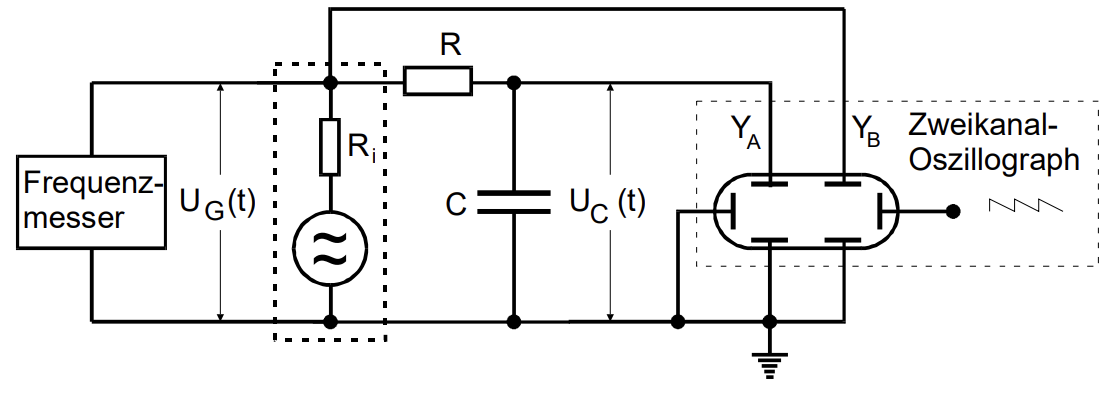
\includegraphics[width=\textwidth]{v353_Schaltkreise_5.png}
    \caption{Schaltkreis des Experimentes}
    \label{fig:Schaltkreis5}
\end{figure}


\section{Versuchsdurchführung}
Zu Beginn wird der Entladevorgang des RC-Kreises beobachtet und vermessen. Für einen nichtgestörten und wiederholten
Entladevorgang wird am Frequenzgenerator eine Rechteckspannung eingestellt. So wird der Kondensator während des Hochs 
geladen und während des Tiefs entladen.

\begin{figure}[H]
    \begin{minipage}[t]{0.5\textwidth}
        Auf dem Oszilloskop wird lediglich der Spannungsverlauf am Kondensator angezeigt. Der passende Messbereich
        wird per Hand eingestellt, sodass die Entladekurve wie in \autoref{fig:Entladekurve} angezeigt wird.
        So kann man die Spannung, in Abhängigkeit der Zeit ablesen. Aus diesen Messwerten wird im Anschluss eine lineare 
        Ausgleichsgerade erstellt.
    \end{minipage}
    \begin{minipage}[t]{0.4\textwidth}
        \vskip-\ht\strutbox
        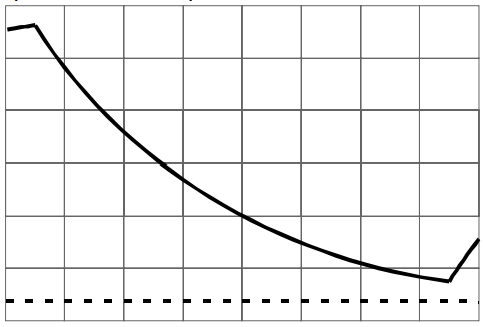
\includegraphics[width=\textwidth]{v353_Entladekurve.png}
        \caption{Skizze der Entladekurve}
        \label{fig:Entladekurve}
    \end{minipage}
\end{figure}
\noindent
Die Ausgleichsgerade besitzt die Steigung
\begin{equation}
    m =  - \frac{1}{RC}.
    \label{eqn:Steigung}
\end{equation}
So wird die gesuchte Konstante $RC$ aus den Messdaten bestimmt.
Eine weitere Methode $RC$ zu bestimmen, ist es die Spannungsamplitude in Abhängigkeit von der Frequenz zu Messen.
Über Gleichung \autoref{eqn:Amplitude} ist es damit möglich die Zeitkonstante zu bestimmen.
Ebenfalls ist es möglich über die Phasenverschiebung $\varphi$ der Spannungen mit Hilfe von Gleichung \autoref{eqn:Amplitude} 
die Zeitkonstante $RC$ zu berechnen.
Beide Methoden werden mit einem Messaufbau durchgeführt.
So wird eine sinusförmige Spannung vom Frequenzgenerator abgegriffen und mit der Kondensatorspannug auf auf dem Oszilloskop 
angezeigt. 
Es wird eine Reihe an verschiedenen Frequenzen durchgegangen. Bei jeder Frequenz wird die Spannungsamplitude $A$ am 
Kondensator und der Phasenabstand $a$ zwischen den angezeigten Spannungen gemessen. Der Phasenabstand ist der Abstand, 
der zwischen den Perioden von Eingangsspannung und Ausgangsspannung liegt.
Die Phasenverschiebung wird durch

\begin{align}
    \varphi = \frac{a}{b} \cdot 2 \pi & & \text{ ,wobei } & b = T = \frac{1}{f}
    \label{eqn:Phase}
\end{align}

\noindent
berechnet.


\section{Messwerte}

Bei der Entladungsmessung des Kondensators wurden 19 Messwerte aufgenommen.
Am Anfang der Entladung ist die Änderungsrate der Kondensatorspannug noch sehr hoch. Daher ist dort das Messintervall kleiner.

\begin{table}[H]
\centering
\caption{Messwerte der Kondensatorentladung.}
\sisetup{table-format=1.1, per-mode=reciprocal}
\begin{tblr}{colspec = {S S[table-format=2.1]}, row{1} = {guard, mode=math},
    }
\toprule
t \mathbin{/} \unit{\milli\second} &
U \mathbin{/} \unit{\volt} \\
\midrule
0       &     11.2  \\
0.2     &     10    \\
0.4     &     8.8   \\
0.5     &     8.4   \\
0.6     &     8.2   \\
0.8     &     7.4   \\
1       &     6.8   \\
1.5     &     5.2   \\
2       &     4     \\
2.5     &     3.2   \\
3       &     2.4   \\
3.5     &     1.6   \\
4       &     1.2   \\
4.5     &     0.8   \\
5       &     0.6   \\
5.5     &     0.4   \\
6       &     0.2   \\
6.5     &     0.1   \\
8.2     &     0     \\
\bottomrule
\end{tblr}
\label{tab:t-U}
\end{table}

\noindent
Um $RC$ über $\varphi$ zu bestimmen, müssen sowohl große, als auch kleine Werte für f 
angenommen werden. Dies wurde nicht gemacht. In der Diskussion wird näher darauf eingegangen.
\begin{table}[H]
    \centering
    \caption{Messwerte der Kondensatorentladung.}
    \sisetup{table-format=1.1, per-mode=reciprocal}
    \begin{tblr}{colspec = {S[table-format=6.0] S[table-format=3.0] S[table-format=3.1]}, 
        row{1} = {guard, mode=math},
        }
    \toprule
    f \mathbin{/} \unit{\hertz} &
    A \mathbin{/} \unit{\volt} &
    a \mathbin{/} \unit{\micro\second} \\    
    \midrule
    1000    &   440     &    260    \\    
    1125    &   240     &    220    \\    
    2500    &   110     &    100    \\    
    5000    &   95      &    50     \\
    7500    &   64      &    32     \\
    10000   &   56      &    24     \\
    15000   &   32      &    17     \\
    30000   &   16      &    14     \\
    50000   &   10      &    5      \\
    100000  &   5       &    2.6    \\    
    \bottomrule
    \end{tblr}
    \label{tab:f-A-a}
    \end{table}




\end{document}

